\chapter{The CMS Detector at the Large Hadron Collider}
\label{chap:CMS}

The CMS detector is a general purpose particle detector that measures the energy and momentum of particles produced in the collision of high-energy protons in the Large Hadron Collider (LHC) at CERN \cite{collaborationCMSExperimentCERN2008}. It was designed with the goal of studying a wide range of physics phenomena, including the study of the electroweak sector, vector-boson scattering, precision studies of the standard model (SM), heavy-ion physics, and searches for physics beyond the SM. The CMS detector is cylindrical, with an overall diameter of $15.0 \text{ m}$, a length of $28.7 \text{ m}$ and a total width of $14,00\text{ m}$. A schematic of the CMS detector is shown in Figure \ref{fig:cms_detector}. Starting from the innermost subsystem of the detector, CMS is composed of the Silicon Tracker, the Electromagnetic and Hadron Calorimeters (ECAL and HCAL respectively), the super-conducting solenoid, and the muon system. Much of the following description of the CMS detector in this chapter is based on the comprehensive design overview provided in the CMS experiment technical paper \cite{collaborationCMSExperimentCERN2008} and \cite{collaborationDevelopmentCMSDetector2024}.

\begin{figure}[ht]
	\centering
	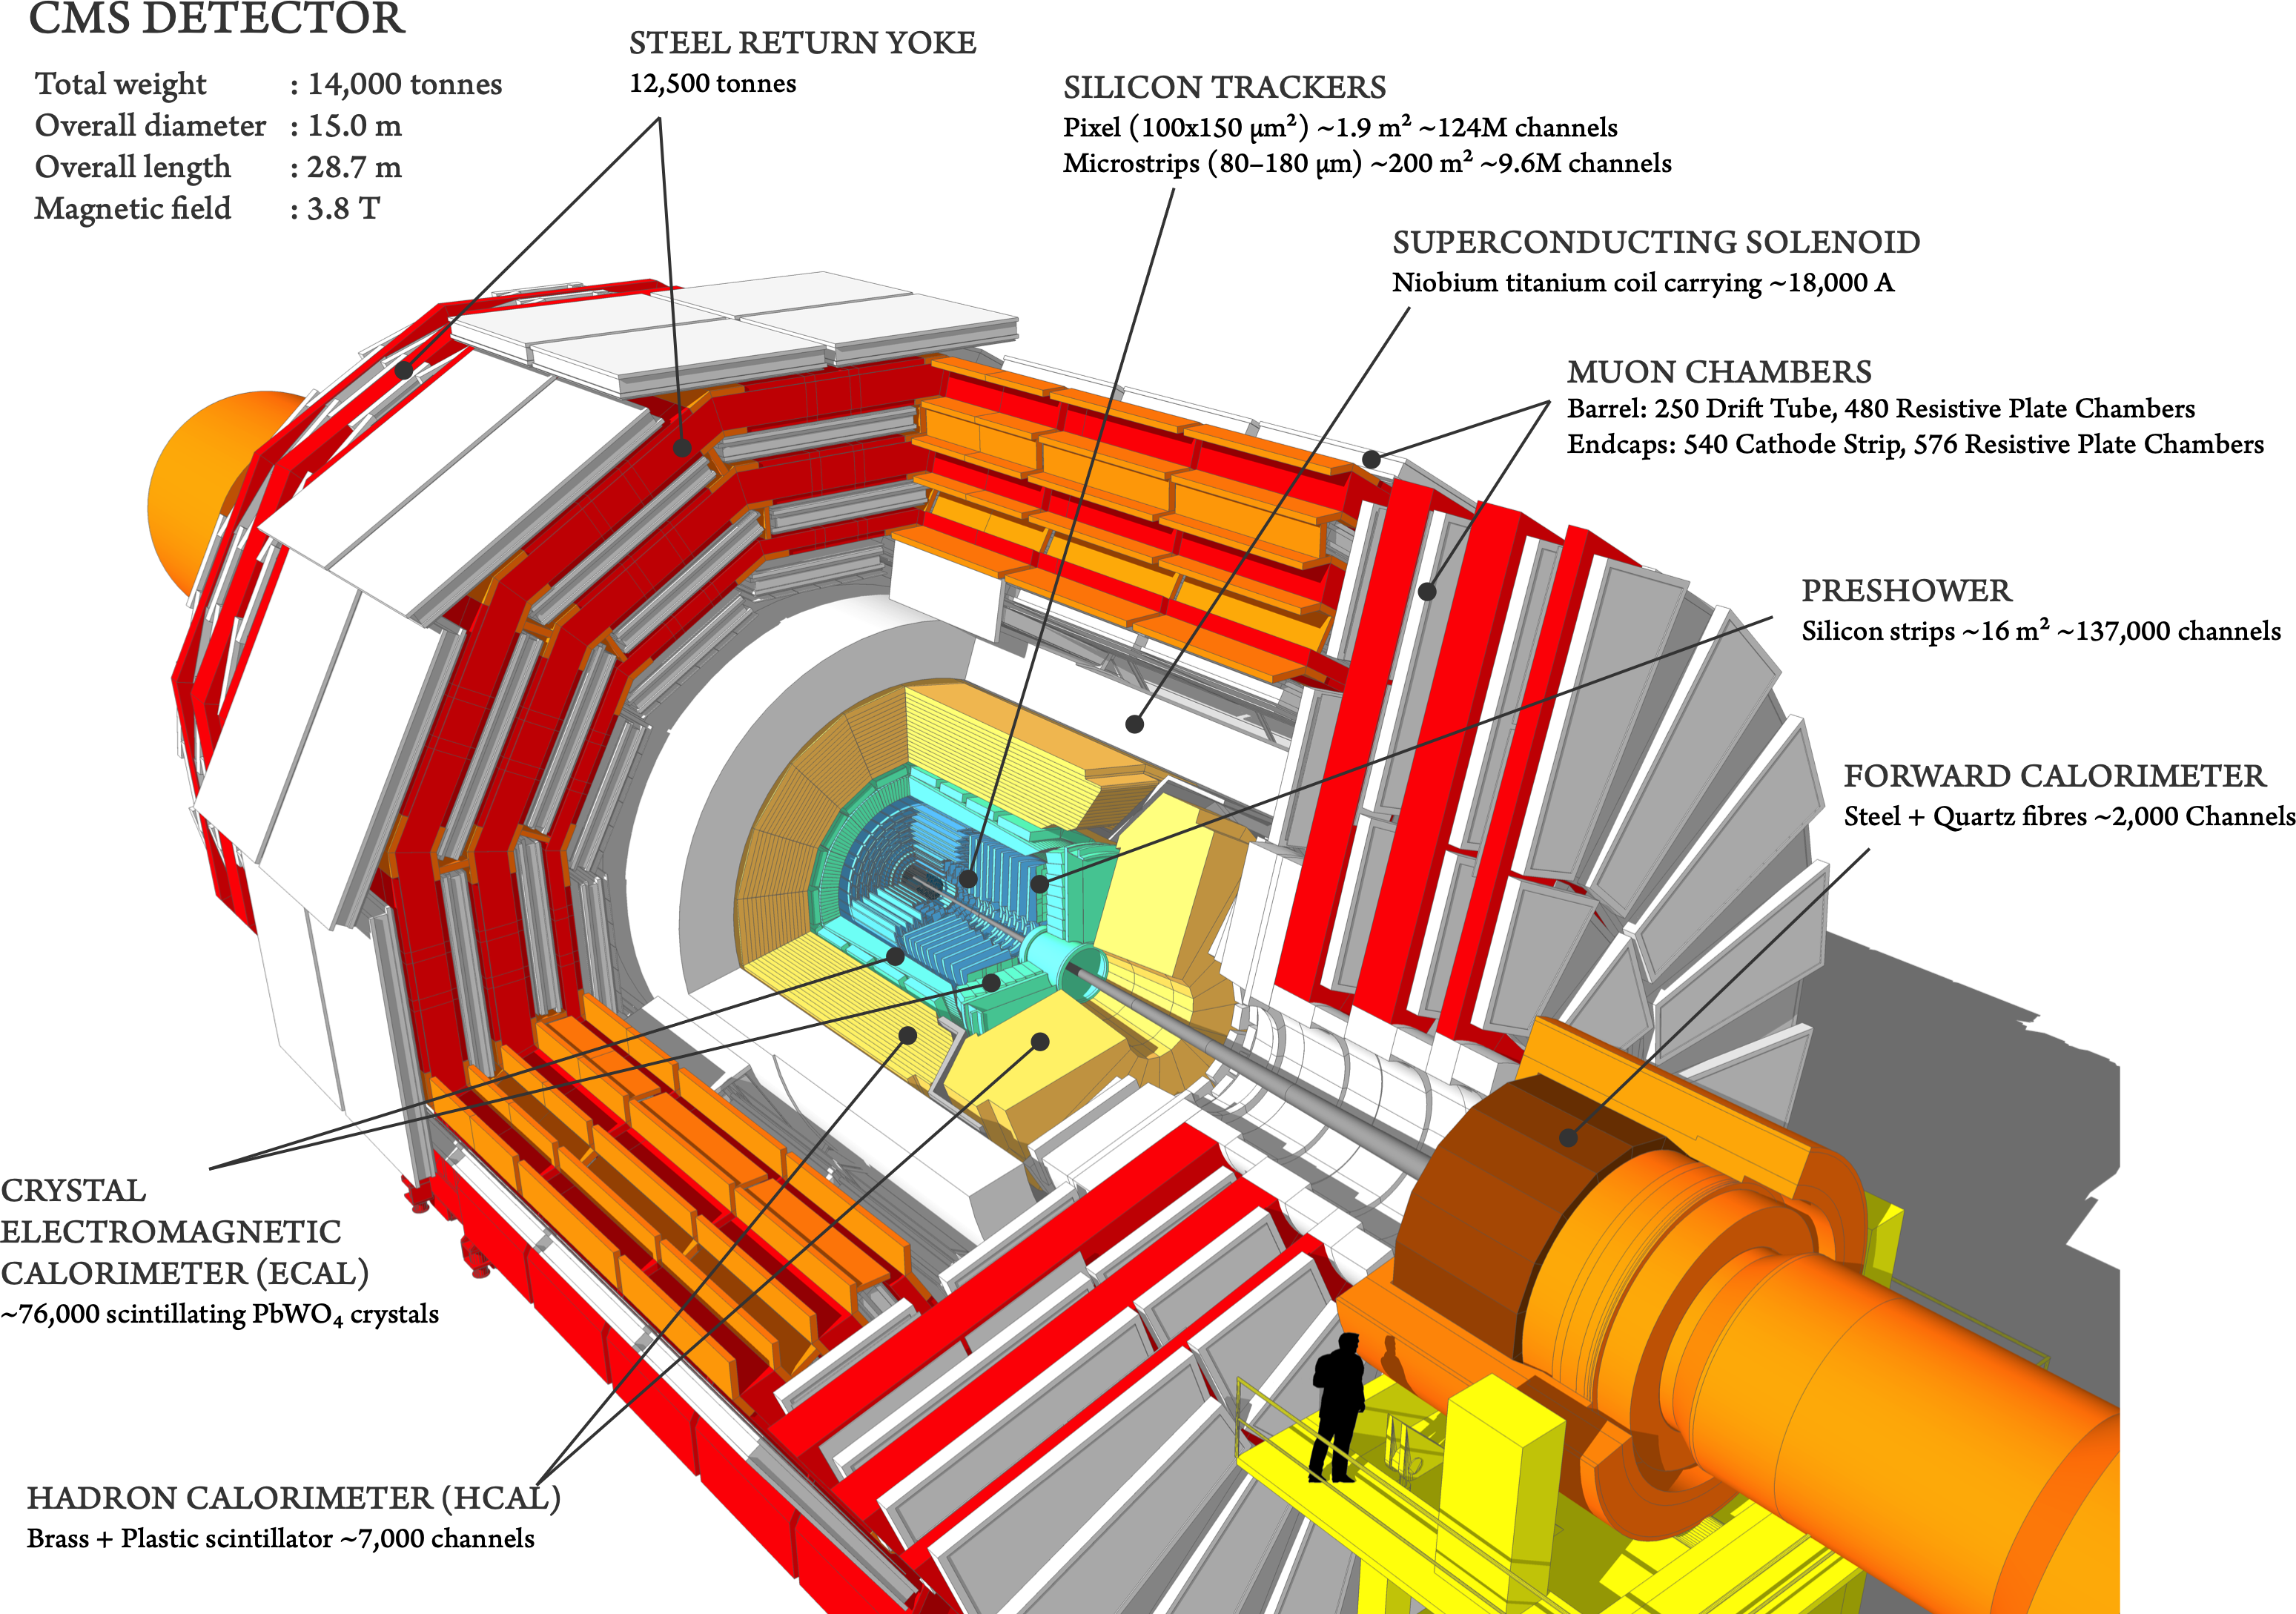
\includegraphics[width=0.8\textwidth]{images/cms_detector.png}
	\caption{Schematic of the CMS detector at the Large Hadron Collider.}
	\label{fig:cms_detector}
\end{figure}

\section{Silicon Tracker}
\label{sec:tracker}

At the heart of the CMS detector is the Tracker system, which is the innermost subsystem. The Tracker is made up of pixel and strip detectors and is responsible for measuring the path of electrically charged particles. This subsystem was designed to offer high precision in the measurement of particle trajectories, allowing for an accurate reconstruction of the primary and secondary vertices. In general, the tracker volume has a length of $5.8 \text{ m}$ and a diameter of $2.5 \text{ m}$. As charged particles go through this volume, their path is bent by the homogeneous magnetic field of $4 \text{ T}$ provided by the CMS solenoid. The curvature of their tracks allows for an accurate measurement of the momentum of the particles. It offers excellent momentum resolution and track efficiency, allowing measurement of $p_{\text{T}}$ down to $50 \text{MeV}$ in the range of $|\eta| < 2.5$. 

The tracker employs a two-layered structure: an inner section composed of silicon pixel layers, surrounded by a larger system of silicon strip layers with coarser segmentation, a structure which is illustrated in Figure \ref{fig:trackquad}. The sensors in both systems are made from doped silicon. When an energetic charged particle goes through a silicon sensor, it generates electron-hole pairs that drift in opposite directions within the semiconductor, producing a measurable current.

\begin{figure}
    \centering
    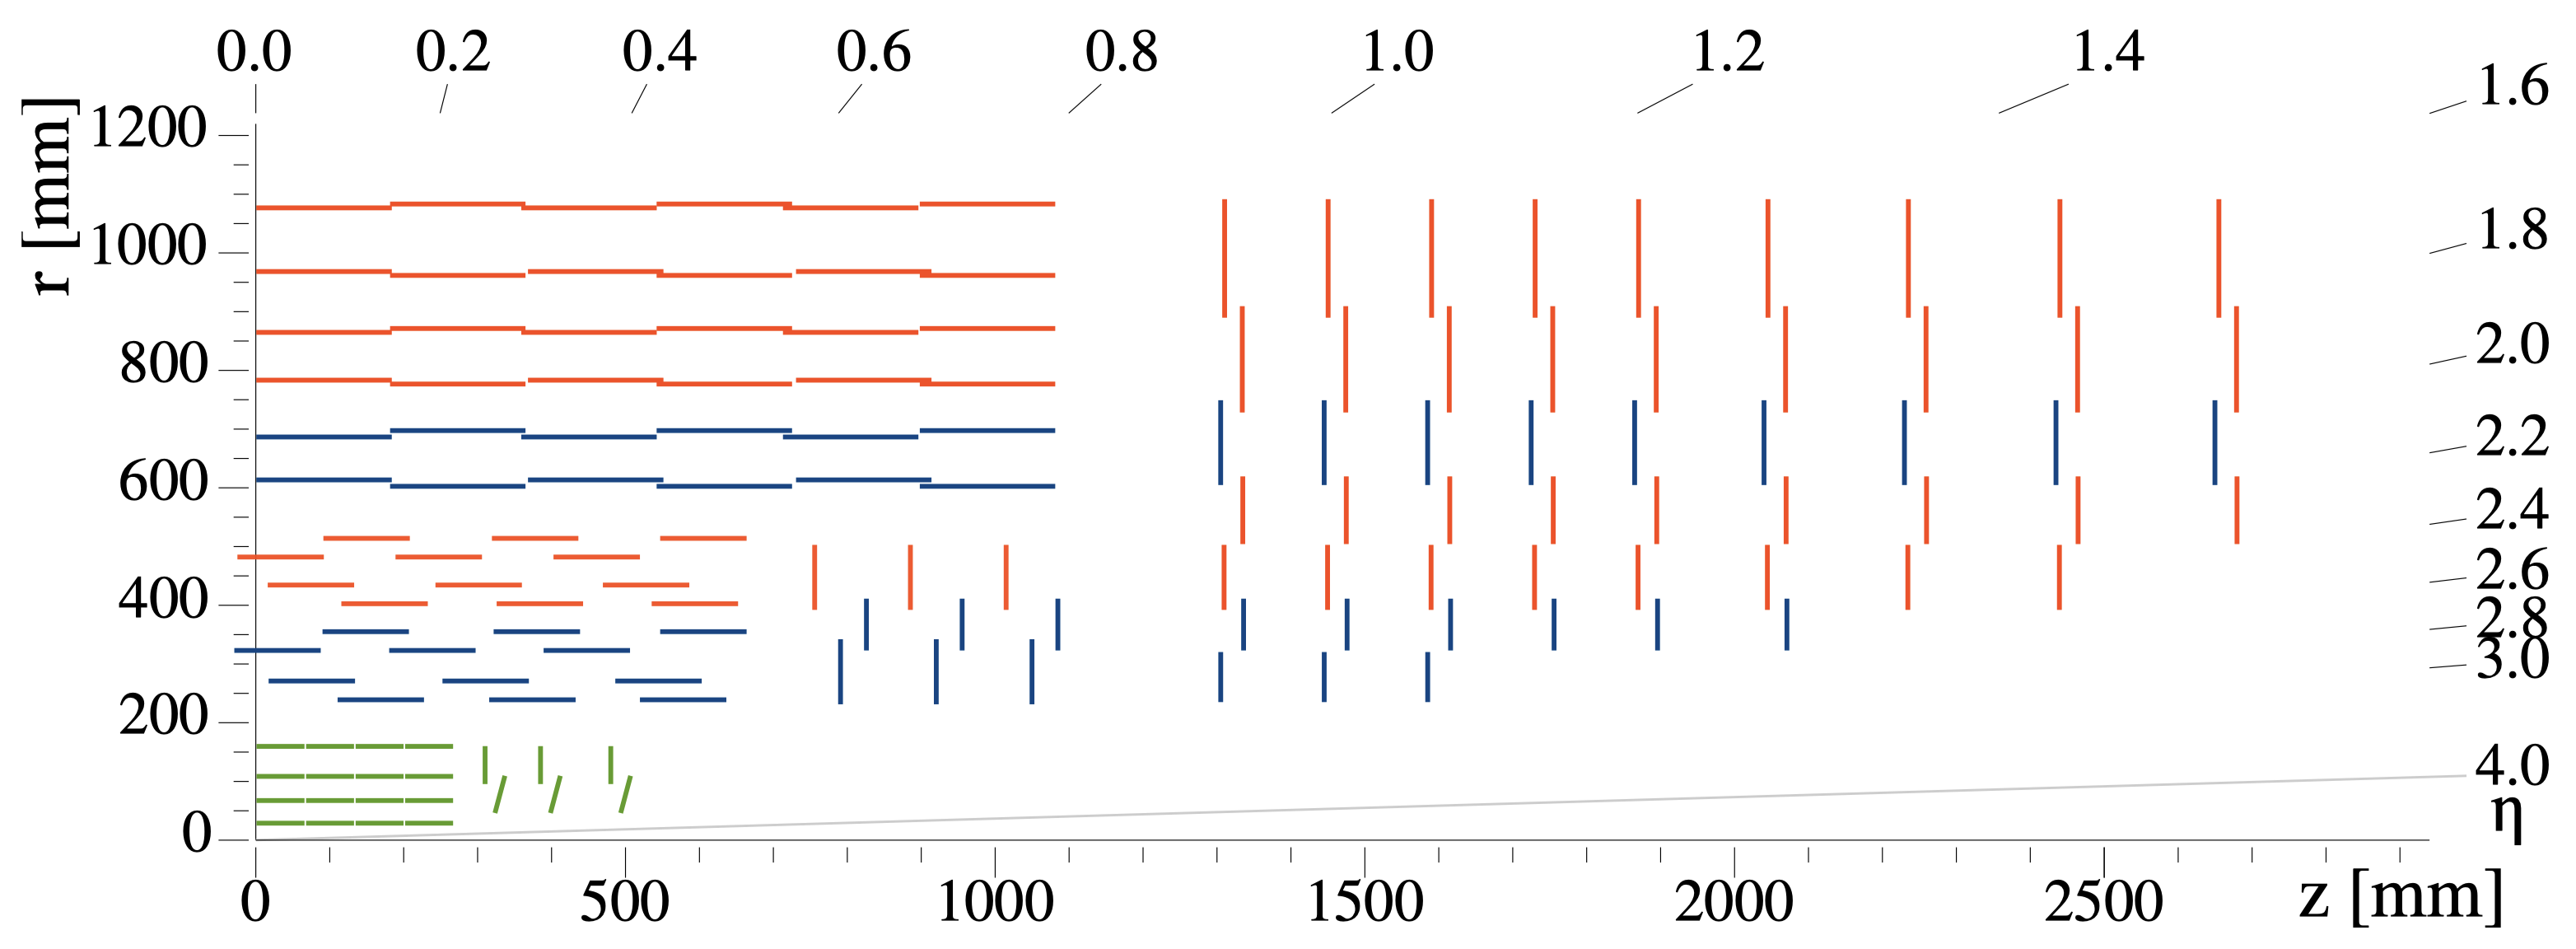
\includegraphics[width=0.85\linewidth]{images/trackquadrant.png}
    \caption{View of a quadrant of the $r-z$ view of the CMS tracker \cite{CERN-LHCC-2017-009}}
    \label{fig:trackquad}
\end{figure}

The Pixel detector consists of four barrel layers with, with the innermost layer of the pixel module sitting just $29 \text{ mm}$ from the beam line. The forward component of the sub-detector consists of 12 half-disks with radii between $45 \text{ mm}$ and $161 \text{ mm}$. Both of these elements, the forward pixel disks (FPIX) and pixel barrel (BPIX) are made up of silicon sensor modules made of a sensor with $160\times416$ pixels connected to 16 read out chips (ROCs), totaling $1184$ modules for the BPIX and $672$ for the FPIX, providing $124$ million read out channels. 

Surrounding the pixel tracker, the silicon strip tracker is divided into an inner barrel, inner disks, outer barre, and outer endcaps. The strip sensors use a p-on-n doping structure and vary in thickness from $320 \;\mu\text{m}$ and $500 \;\mu\text{m}$. Compared to the pixel tracker, the strip sensors are significantly larger. Their dimensions range from $6\text{ cm} \times 12 \text{ cm}$ to $10\text{ cm} \times 9 \text{ cm}$. The full strip system comprises 34 layers (barrel and endcap combined, encompassing about $200 \text{ m}^2$ of silicon, and typically delivers nine or more spatial measurements per track with $|\eta|<2.4$.

Together, the pixel and strip detectors enable for detailed tracking of charge particles. Around $|\eta| = 0$, the transverse impact parameter resolution is $10-100 \;\mu\text{m}$, while the longitudinal resolution is $40-140 \;\mu\text{m}$.

\section{Electromagnetic Calorimeter}
\label{sec:ECAL}

The electromagnetic calorimeter (ECAL) is designed to measure the energy of photons and particles with electric charge, and it encloses the silicon tracker. It is composed of lead tungstate ($\text{PbWO}_4$) crystals that scintillate when energetic charged particles pass through it, producing light that is detected by external photodetectors (avalanche photodiodes in the barrel, vacuum phototriodes in the endcaps). It is made up of a barrel and an endcap, both of which are composed of similarly shaped tapered prisms with dimensions $2.2\text{ cm}\times2.2\text{ cm}\times23\text{ cm}$ in the barrel, and $3\text{ cm}\times3\text{ cm}\times22\text{ cm}$ in the barrel. The barrel consists of 35 supermodules that house a total of $61,200$ crystals covering $|\eta| <1.479$, while the endcaps include $14,648$ covering $1.479 <|\eta|<3.0$. In front of the endcap crystals, a preshower detector with two planes of silicon strip sensors measuring $61\times1.9\text{ mm}^2$ interleaved with lead absorbers is used at $1.65 <|\eta|<2.6$ to enhance spatial resolution, allowing for improved identification of neutral pions through the resolution of photon pairs.

\section{Hadronic Calorimeters}
\label{sec:HCAL}

The hadronic calorimeter (HCAL) is designed to measure the energy of particles, particularly hadrons, that are not entirely absored by the ECAL. It is composed of four main components: the hadron barrel (HB) inside the magnet coil, hadron endcap (HE), hadron outer (HO) and hadron forward (HF) calorimeters. The HCAL's pseudorapidity span is $|\eta| <5.2$. As a sampling calorimeter, it has thick absorber layers to initiate particle showers and interleaved thin scintillating layers for energy detection and signal readout. It contains $61,200$ lead tungstate crystals in the barrel, and $7,324$ crystals at each endcap, with a preshower detector placed in front of the latter group of crystals.

The HB covers a range of $|\eta| <1.3$ and extends radially from the outer edge of the ECAL to the inner boundary of the solenoid magnet. The absorber structure consists of fourteen layers cartridge brass, separated by structural steel plates, yielding $75 \text{ cm}$ of material. Between the brass layers, $3.7 \text{ mm}$ sheets of Kuraray SCSN-81 plastic scintillator are inserted, and an initial $9 \text{ mm}$ layers of Bicron BC408 scintillator is placed at the front. The resulting segmentation in both $\eta$ and $\phi$ is 0.087. The light emitted by the scintillators is captured by optical fibers and transmitted to hybrid photodiodes for detection.

The HE covers the angular region $1.3 <|\eta| < 3$. It has a similar configuration as the HB, with brass as the absorber material and SCSN-81 and BC408 scintillators as the active media. These are offset to ensure full spacial coverage.

The HO complements the HB by adding additional depth in the $|\eta| <1.3$ range, compensating for the radial space constraint imposed by the solenoid. It uses scintillator layers placed beyond the magnet, and the scintillator elements consist of 10 mm thick BC408 tiles, arranged with 0.087 granularity in $\eta$ and $\phi$, and read out via optical fiber.

The HF calorimeters extend the HCAL coverage to the forward region, spanning $3 <|\eta|<5.2$, and are located $11.2 \text{ m}$ from the interaction point. This region experiences a significantly higher particle flux compared to the rest of the HCAL components to particles with forward momentum, requiring greater radiation tolerance. The absorber consists of $165 \text{ cm}$ of steel. Quartz fibers generate Cherenkov radiation from charged particles within the shower. Half of the fibers are embedded starting $22 \text{ cm}$ from the detector's front to differentiate early EM showers from dee-penetrating hadronic ones, whereas the rest span the full detector length. These fibers are grouped into readout towers with segmentation $\Delta \eta \times \Delta \phi = 0.175\times0.175$, and the signal is detected using photomultiplier tubes.

\section{Muon System}
\label{sec:muon}

Muons, being heavier than electrons, have experience significantly lower Bremsstrahlung when traversing the material in the detector, and are thus less likely to be absorbed by the calorimeters and can even cross the solenoid. To account for this, there are three dedicated detectors within and surrounding the flux return yoke. These detectors are the drift tubes (DTs) in the barrel region, the cathode strip chambers (CSCs) in the endcaps, and the resistive plate chambers (RPCs) which are in both the endcaps and the barrel, make up the Muon system.

The three detector types in the Muon system operate under the same principle: a gas mixture is contained in an electric field and, when a muon traverses the gas, it ionizes the atoms, producing an electron cascade due to the high voltage ($3500 \text{ V}$ for DTs and CSCs, $9000 \text{ V}$ for RPCs).

There are a total of 250 DTs, providing a coverage of $|\eta| <1.2$. Each one features a central wire anode and a side cathode, with a rectangular cross-section of $13 \text{ mm}$ by $42 \text{ mm}$. They are layered in staggered formation and alternately oriented to obtain position measurements along the $r-\phi$ and $z$ axes. Based on drift time, the spatial resolution of a single DT is around $170 \;\mu\text{m}$, yielding an overall resolution of approximately $100 \;\mu\text{m}$ when combining multiple layers.

There are 468 CSCs in the endcaps which cover an interval of $0.9 <|\eta|< 2.4$. They are made up of six gas-filled gaps formed by alternating cathode strip and anode wire planes. The wires run along the azimuthal direction, while the strips are radial, allowing for two-dimensional position information.

The RPCs, installed on both the barrel and endcap region, cover $|\eta| <1.6$. They consist of parallel gas gaps that sandwich readout strips. They can provide timing information faster than the LHC bunch crossing rate, and readout is handled by front-end boards that transmit data to the trigger system via optical links at a bandwidth of $1.6\text{ GHz}$.

\section{Trigger System}
\label{sec:triggers}

In CMS, a single event corresponds to a bunch crossing, which takes place at $40 \text{MHz}$. The information from each event corresponds to $\~ 1\text{ MB}$ of data, which means that recording every event would require an unrealistic data flow of the $\~ 50\text{TB/s}$. However, most events result in a well-understood QCD phenomenon or in mostly low-momentum transfer between the colliding protons, so it is not only not feasible, but also not desirable, to store all of this data. In order to address this, CMS uses a two-layer trigger system to record only those events which may contain interesting physics.

The first stage of CMS's trigger system is the Level-1 Trigger (L1T). In this stage, reduced-resolution event information is fed into selection algorithms implemented in specialized hardware such as FPGAs and ASICs, allowing fast decision-making at a rate of up to $100\text{ kHz}$. The L1T integrates information only from the ECAL, HCAL and the three muon systems to identify coarse particle signatures and global event features, such as total transverse energy and missing energy. This is done in multiple stages: first, the detector signals from these subsystems are preprocessed into trigger primitives (TPs) with limited granularity. The CSC, RPC and DT TPs are processed and goo through muon track finder algorithms, the output of which are passed to a global muon trigger. The ECAL and HCAL TPs are fed through two layers of calorimeter triggers. The output from the Global Muon Trigger and the Calorimeter triggers is then passed to a Global Trigger, which makes the final decision and applies prescales (PS) if there are any to apply.

The High Level Trigger (HLT) is the second layer in CMS's triggering system, and it uses more advanced selection algorithms which are implemented in software, further reducing the events selected by the L1T to $1\text{kHz}$. The reconstruction algorithms this system uses are a simplified version of the offline reconstruction algorithms and, in contrast to the L1T system, the HLT integrates inputs from all detector subsystems. All this processing is done in a dedicated computing form with up to $30,000$ CPUs.

\section{Detector \& Data Quality Monitoring}
\label{sec:dqm}

To ensure that the data from the CMS detector are of the utmost quality for the many physics analyses, there are Data Quality Monitoring (DQM) and Data Certification (DC) groups that monitor the health of the different subsystems of the CMS detector, as well as the integrity of the data. These groups conduct their monitoring during live data-taking (i.e., "online" operations) and also after the data have been fully reconstructed (i.e., "offline" operations). During Online DQM, live monitoring is performed on the status of the detector using quickly processed data in order to identify problems as soon as they appear. On the other hand, Offline DQM takes place hours afterward. During this second phase, experts evaluate a more thoroughly processed version of the same data seen in Online DQM, giving them access to more granular information on the performance of the detector and the quality of the physics reconstruction. Through this process, they provide certification flags that indicate whether or not the data pass the quality check for their particular subsystem and could be used for physics analysis. In addition, Offline experts can provide feedback to the Online crew of issues which they might have missed.

The data in both Online and Offline DQM is visualized through a platform dubbed DQMGUI (DQM Graphical User Interface). A screen capture showing an example run (run number 380238) is shown in Figure \ref{fig:dqmgui}. This platform shows a large collection of different plots and histograms, named monitoring elements, each showcasing a particular aspect of the detector (e.g., number of read-out chips in the Pixel detector) or physics reconstruction (e.g., track $p_T$ distributions). The data shown in these monitoring elements constitute a summary of what occurred during a given run, where a run is a continuous data-taking time period with particular data-taking conditions. These runs can be further subdivided into lumisections (LSs), which are periods of 23.3 seconds of data taking. Thus, most monitoring histograms result from the integration of the data over all LSs of the run, which can be made up of upwards of \~2000 LSs for the longest runs.

\begin{figure}
    \centering
    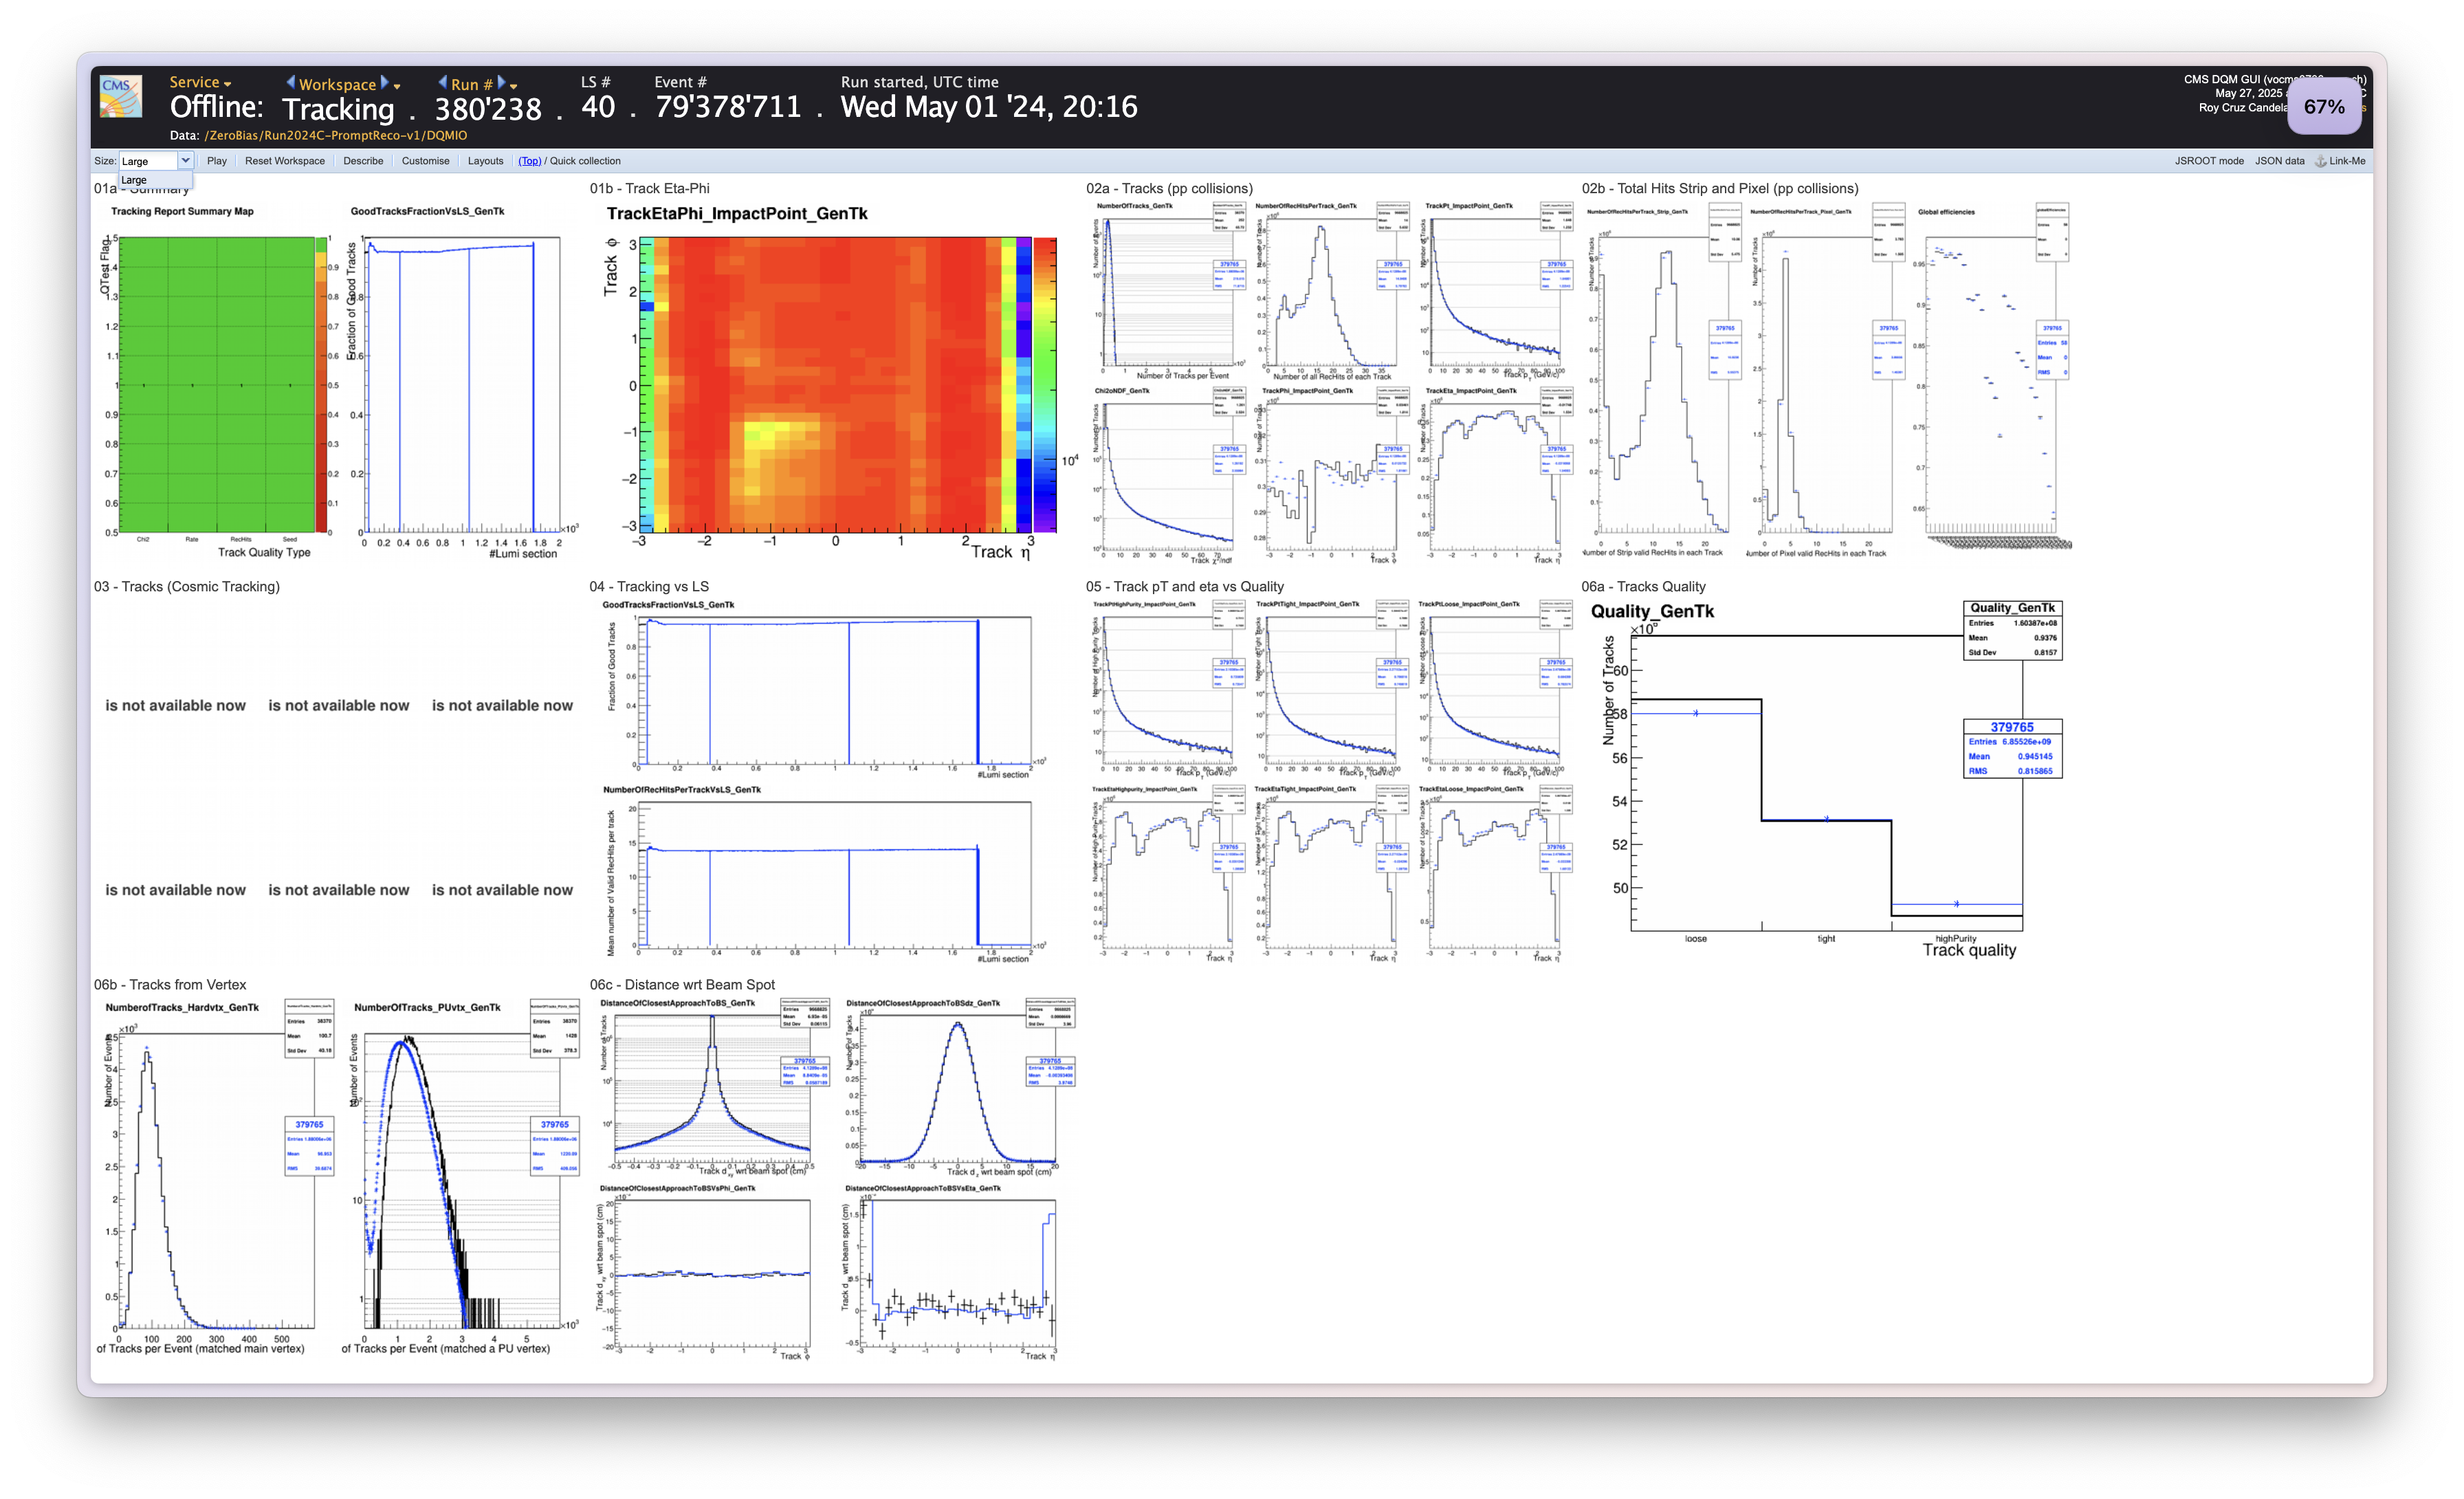
\includegraphics[width=0.8\linewidth]{images/dqmgui.png}
    \caption{Capture of example visualization of run 380238 in the DQMGUI}
    \label{fig:dqmgui}
\end{figure}